% ****************************************************************************************************
\chapter{Proof of Concept -- Using the Example of SAP HANA Cloud}\label{ch:poc}
% ****************************************************************************************************

In order to evaluate and show the applicability of the previous developed \ac{DSR} artifacts -- classification scheme (cf. Chapter \ref{ch:sota}), \ac{CLD} (cf. Chapter \ref{ch:cld}), and \ac{SFD} (cf. Chapter \ref{ch:sfd}) --, in the following a \acf{PoC} study using the example of the SAP HANA Cloud platform is presented. This approach is in conformity with the \ac{DSR} design cycle of \citet[pp. 88,90-91]{Hevner2007} and the \ac{DSR} activity evaluation according to \citet[p. 56]{Peffers2007}, whereby the artifacts have been evaluated against the real world by their reapplication in the context of \ac{PaaS} business models.

% ****************************************************************************************************
\section{Business Model Design Elements}\label{ch:poc:cs}
% ****************************************************************************************************
The business model of the SAP HANA Cloud platform is explained and illustrated, using the business model conceptualization proposed by \citet{Johnson2008}, in detail within Subsection \ref{ch:sota:sap}. In order to classify \ac{PaaS} business models, a corresponding classification scheme have been developed. How the SAP HANA Cloud platform addresses the identified classification criteria is briefly discussed below and illustrated in Figure \ref{fig:cs:sap} by means of a morphological box, whereas the addressed characteristics are highlighted.

Within the case study analysis of this platform, four diverse stakeholder groups, which are directly targeted, were identified -- application customer, development partners, platform customers, and individual developers. Using the classification scheme terminology, the SAP HANA Cloud platform addresses all five identified customer segments -- \ac{IT} startup, \ac{SI}, \ac{ISV}, platform customer, as well as application customer. However, these customer segments are served differently as illustrated further below. SAP HANA Cloud aims to support the development, deployment, and management of standalone as well as integrated cloud applications. However, the focus of this platform is rather to provide extensive integration features und thus classified as \ac{PaaS} platform with the core value proposition integration. The SAP HANA Cloud platform is neither an open source platform nor a highly regulated platform, hence a partly limited governance model is pursued. Meaning platform users of all characteristics have an extensive freedom of choice, although certain areas are regulated directly by the platform provider. Even though the SAP HANA Cloud platform is offering several technical capabilities, for instance the SAP Hana Cloud Eclipse plugin and corresponding \ac{SDK} (Java), they are considered rather as limited and thus for the criterion technical scope the characteristic limited technical capabilities is selected. In particular, the comparison with other \ac{PaaS} platforms and their technical capabilities support this classification. Based on the SAP HANA Cloud platform case study, three revenue streams which are used by this platform have been identified. First, platform customers are charged with subscription-based fees ranging from $370$ to $16.000$ \ac{EUR} monthly. Second, SAP takes a revenue share of $15\%$ for platform modules developed by complementors -- \acp{ISV} and \ac{IT} -- and distributed over the SAP store. Third, various charged addition services are offered, including annual development partner fees of $1.990$ \ac{EUR} and application certification fees ranging from $495$ to $990$ \ac{EUR}.

\begin{figure}[tb]
	\centering
	% ****************************************************************************************************
% Classification Scheme SAP
% ****************************************************************************************************

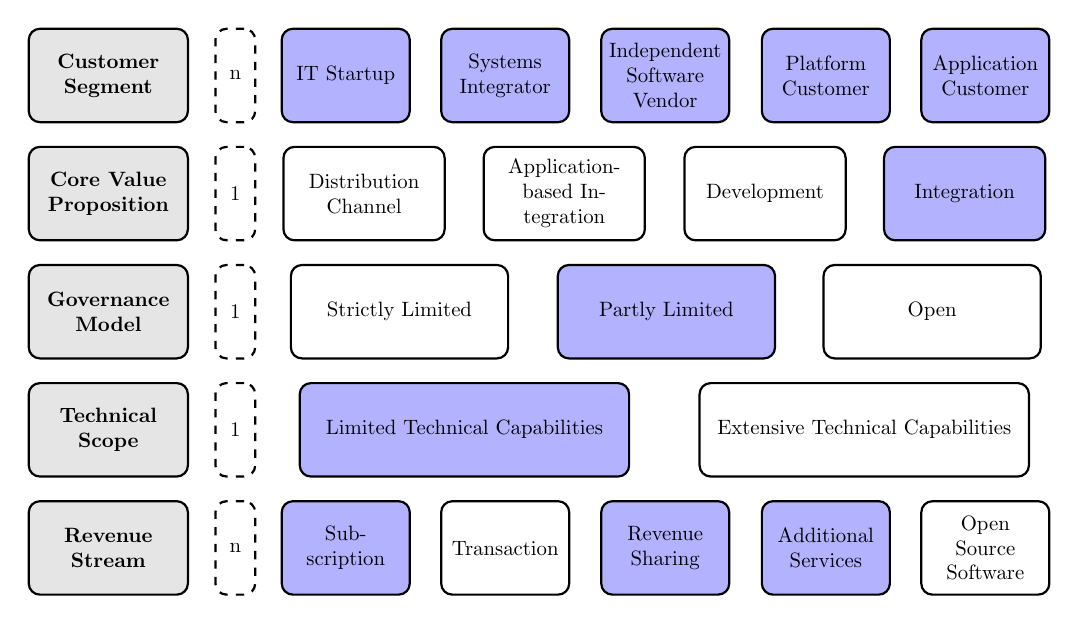
\begin{tikzpicture}[scale=0.75, every node/.style={scale=0.75}]

\node[font={\bfseries},draw,text width=7em,text centered,rectangle,rounded corners,minimum height=4.5em,thick,fill=gray!20] (1) at (-1,8) {Customer Segment};
\node[font={\bfseries},draw,text width=7em,text centered,rectangle,rounded corners,minimum height=4.5em,thick,fill=gray!20] (1) at (-1,6) {Core Value Proposition};
\node[font={\bfseries},draw,text width=7em,text centered,rectangle,rounded corners,minimum height=4.5em,thick,fill=gray!20] (1) at (-1,4) {Governance Model};
\node[font={\bfseries},draw,text width=7em,text centered,rectangle,rounded corners,minimum height=4.5em,thick,fill=gray!20] (1) at (-1,2) {Technical Scope};
\node[font={\bfseries},draw,text width=7em,text centered,rectangle,rounded corners,minimum height=4.5em,thick,fill=gray!20] (1) at (-1,0) {Revenue Stream};

\node[draw,text width=1.25em,text centered,rectangle,rounded corners,minimum height=4.5em,thick,dashed] (1) at (1.15,8) {n};
\node[draw,text width=1.25em,text centered,rectangle,rounded corners,minimum height=4.5em,thick,dashed] (1) at (1.15,6) {1};
\node[draw,text width=1.25em,text centered,rectangle,rounded corners,minimum height=4.5em,thick,dashed] (1) at (1.15,4) {1};
\node[draw,text width=1.25em,text centered,rectangle,rounded corners,minimum height=4.5em,thick,dashed] (1) at (1.15,2) {1};
\node[draw,text width=1.25em,text centered,rectangle,rounded corners,minimum height=4.5em,thick,dashed] (1) at (1.15,0) {n};

\node[draw,text width=5.5em,text centered,rectangle,rounded corners,minimum height=4.5em,thick,fill=blue!30] (1) at (3.02,8) {IT Startup};
\node[draw,text width=5.5em,text centered,rectangle,rounded corners,minimum height=4.5em,thick,fill=blue!30] (1) at (5.72,8) {Systems Integrator};
\node[draw,text width=5.5em,text centered,rectangle,rounded corners,minimum height=4.5em,thick,fill=blue!30] (1) at (8.43,8) {Independent Software Vendor};
\node[draw,text width=5.5em,text centered,rectangle,rounded corners,minimum height=4.5em,thick,fill=blue!30] (1) at (11.15,8) {Platform Customer};
\node[draw,text width=5.5em,text centered,rectangle,rounded corners,minimum height=4.5em,thick,fill=blue!30] (1) at (13.85,8) {Application Customer};

\node[draw,text width=7.1em,text centered,rectangle,rounded corners,minimum height=4.5em,thick] (1) at (3.33,6) {Distribution Channel};
\node[draw,text width=7.1em,text centered,rectangle,rounded corners,minimum height=4.5em,thick] (1) at (6.72,6) {Application-based Integration};
\node[draw,text width=7.1em,text centered,rectangle,rounded corners,minimum height=4.5em,thick] (1) at (10.12,6) {Development};
\node[draw,text width=7.1em,text centered,rectangle,rounded corners,minimum height=4.5em,thick,fill=blue!30] (1) at (13.5,6) {Integration};

\node[draw,text width=9.8em,text centered,rectangle,rounded corners,minimum height=4.5em,thick] (1) at (3.93,4) {Strictly Limited};
\node[draw,text width=9.8em,text centered,rectangle,rounded corners,minimum height=4.5em,thick,fill=blue!30] (1) at (8.45,4) {Partly Limited};
\node[draw,text width=9.8em,text centered,rectangle,rounded corners,minimum height=4.5em,thick] (1) at (12.95,4) {Open};

\node[draw,text width=15.2em,text centered,rectangle,rounded corners,minimum height=4.5em,thick,fill=blue!30] (1) at (5.03,2) {Limited Technical Capabilities};
\node[draw,text width=15.2em,text centered,rectangle,rounded corners,minimum height=4.5em,thick] (1) at (11.8,2) {Extensive Technical Capabilities};

\node[draw,text width=5.5em,text centered,rectangle,rounded corners,minimum height=4.5em,thick,fill=blue!30] (1) at (3.02,0) {Sub-scription};
\node[draw,text width=5.5em,text centered,rectangle,rounded corners,minimum height=4.5em,thick] (1) at (5.72,0) {Transaction};
\node[draw,text width=5.5em,text centered,rectangle,rounded corners,minimum height=4.5em,thick,fill=blue!30] (1) at (8.43,0) {Revenue Sharing};
\node[draw,text width=5.5em,text centered,rectangle,rounded corners,minimum height=4.5em,thick,fill=blue!30] (1) at (11.15,0) {Additional Services};
\node[draw,text width=5.5em,text centered,rectangle,rounded corners,minimum height=4.5em,thick] (1) at (13.85,0) {Open Source Software};

\end{tikzpicture}
	\caption{Proof of Concept -- Classification}
	\label{fig:cs:sap}
\end{figure}

As set out above, the classification scheme developed in this thesis can be easily used to initially assess and classify \ac{PaaS} business models and their characteristics. Whereby the classification scheme is aimed to be as user friendly as possible -- a key classification guideline according to \citet[p. 41]{Fettke2003} -- and thereby ensuring that the classification criteria as well as their characteristics are comprehensible and sufficient.



% zwei modellierungsarten: abolut und relative


\begin{table}[t]
	\centering
	\begin{tabular}{llllllll}
		\toprule 
		\multicolumn{8}{c}{\footnotesize \textbf{Variables and their corresponding Values}} \\ \midrule
		\footnotesize $GOV(t_0)$ & \footnotesize $0.6$ & \footnotesize $CVP_{ITS}(t_0)$ & \footnotesize $0.04$ & \footnotesize $P_{IN_{ITS}}$ & \footnotesize $0.005$ & \footnotesize $P_{IM_{ITS}}$ & \footnotesize $0.01$ \\
		\footnotesize $TS(t_0)$ & \footnotesize $0.5$ & \footnotesize $CVP_{SI}(t_0)$ & \footnotesize $0.03$ & \footnotesize $P_{IN_{SI}}$ & \footnotesize $0.0125$ & \footnotesize $P_{IM_{SI}}$ & \footnotesize $0.025$ \\
		\footnotesize $AS(t_0)$ & \footnotesize $0.4$ & \footnotesize $CVP_{ISV}(t_0)$ & \footnotesize $0.05$ & \footnotesize $P_{IN_{ISV}}$ & \footnotesize $0.005$ & \footnotesize $P_{IM_{ISV}}$ & \footnotesize $0.01$ \\
		& & \footnotesize $CVP_{PC}(t_0)$ & \footnotesize $0.07$ & \footnotesize $P_{IN_{PC}}$ & \footnotesize $0.0125$ & \footnotesize $P_{IM_{PC}}$ & \footnotesize $0.025$ \\
		& & \footnotesize $CVP_{AC}(t_0)$ & \footnotesize $0.01$ & \footnotesize $P_{IN_{AC}}$ & \footnotesize $0.01$ & \footnotesize $P_{IM_{AC}}$ & \footnotesize $0.02$ \\ \bottomrule
	\end{tabular}
	\caption{Proof of Concept -- Simulation Variables}
	\label{tab:mvar:sap}
\end{table}




\begin{figure}[htb]
	\centering
	% ****************************************************************************************************
% Graph Population Customer Segments Stocks
% ****************************************************************************************************

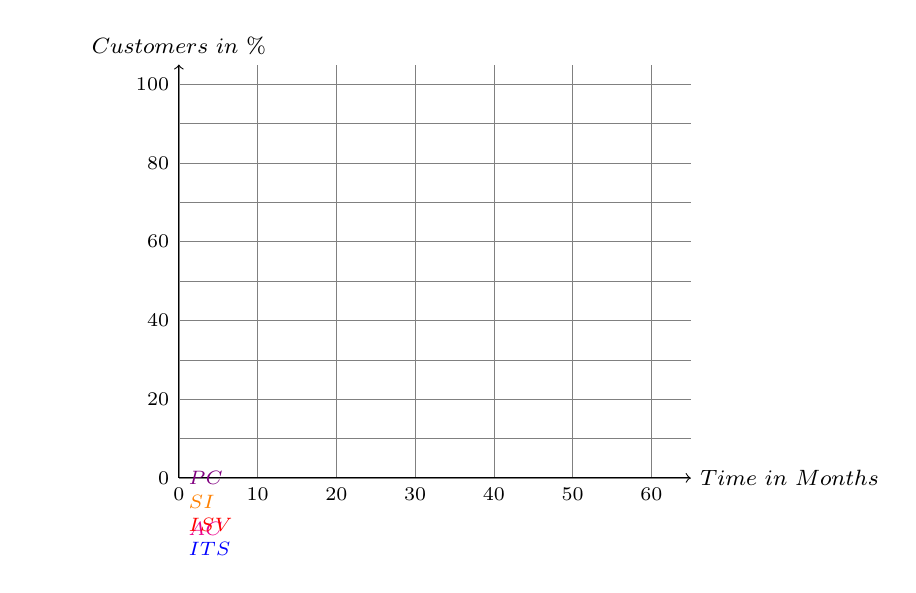
\begin{tikzpicture}[x=0.1cm,y=0.05cm]

  \def\xmin{0}
  \def\xmax{65}
  \def\ymin{0}
  \def\ymax{105}

  % grid
  \draw[style=help lines, ystep=10, xstep=10] (\xmin,\ymin) grid
  (\xmax,\ymax);

  % axes
  \draw[->] (\xmin,\ymin) -- (\xmax,\ymin) node[right] {\footnotesize $Time~in~Months$};
  \draw[->] (\xmin,\ymin) -- (\xmin,\ymax) node[above] {\footnotesize $~~~~~~~Customers~in~\%~~~~~~~$};

  \foreach \x in {0,10,...,60}
    \node at (\x, \ymin) [below] {\scriptsize \x};
  \foreach \y in {0,20,...,100}
    \node at (\xmin,\y) [left] {\scriptsize \y};

  %,mark=*,mark size=0.5pt
	\draw[color=magenta] plot[smooth] file {simulationData/AC/populationAC.txt}
			node [below=0.65cm,right] {\scriptsize $AC$};
	\draw[color=blue] plot[smooth] file {simulationData/ITS/populationITS.txt}
			node [below=0.9cm,right] {\scriptsize $ITS$};	
	\draw[color=red] plot[smooth] file {simulationData/ISV/populationISV.txt}
			node [below=0.6cm,right] {\scriptsize $ISV$};	
	\draw[color=orange] plot[smooth] file {simulationData/SI/populationSI.txt}
			node [below=0.3cm,right] {\scriptsize $SI$};	
	\draw[color=violet] plot[smooth] file {simulationData/PC/populationPC.txt}
			node [right] {\scriptsize $PC$};	
												
\end{tikzpicture}

	\caption{Proof of Concept Simulation -- Customers}
\end{figure}

\begin{figure}[htb]
	\centering
	% ****************************************************************************************************
% Graph Potential Customer Segments Stocks
% ****************************************************************************************************

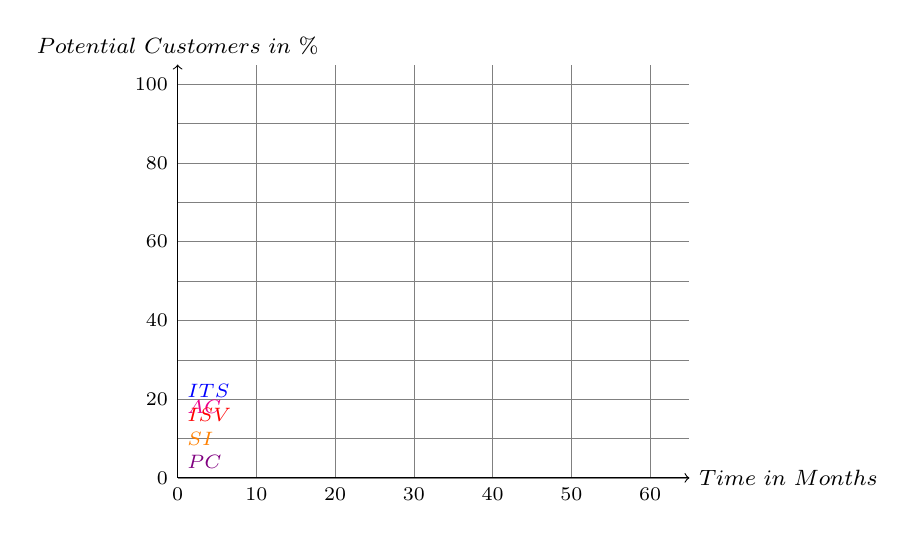
\begin{tikzpicture}[x=0.1cm,y=0.05cm]

  \def\xmin{0}
  \def\xmax{65}
  \def\ymin{0}
  \def\ymax{105}

  % grid
  \draw[style=help lines, ystep=10, xstep=10] (\xmin,\ymin) grid
  (\xmax,\ymax);

  % axes
  \draw[->] (\xmin,\ymin) -- (\xmax,\ymin) node[right] {\footnotesize $Time~in~Months$};
  \draw[->] (\xmin,\ymin) -- (\xmin,\ymax) node[above] {\footnotesize $Potential~Customers~in~\%$};

  \foreach \x in {0,10,...,60}
    \node at (\x, \ymin) [below] {\scriptsize \x};
  \foreach \y in {0,20,...,100}
    \node at (\xmin,\y) [left] {\scriptsize \y};

  %,mark=*,mark size=0.5pt
	\draw[color=magenta] plot[smooth] file {simulationData/AC/potentialAC.txt}
			node [above=0.9cm,right] {\scriptsize $AC$};
	\draw[color=blue] plot[smooth] file {simulationData/ITS/potentialITS.txt}
			node [above=1.1cm,right] {\scriptsize $ITS$};	
	\draw[color=red] plot[smooth] file {simulationData/ISV/potentialISV.txt}
			node [above=0.8cm,right] {\scriptsize $ISV$};	
	\draw[color=orange] plot[smooth] file {simulationData/SI/potentialSI.txt}
			node [above=0.5cm,right] {\scriptsize $SI$};	
	\draw[color=violet] plot[smooth] file {simulationData/PC/potentialPC.txt}
			node [above=0.2cm,right] {\scriptsize $PC$};	
	
													
\end{tikzpicture}

	\caption{Proof of Concept Simulation -- Potential Customers}
\end{figure}

\begin{figure}[htb]
	\centering
	% ****************************************************************************************************
% Graph Overall Adoption 
% ****************************************************************************************************

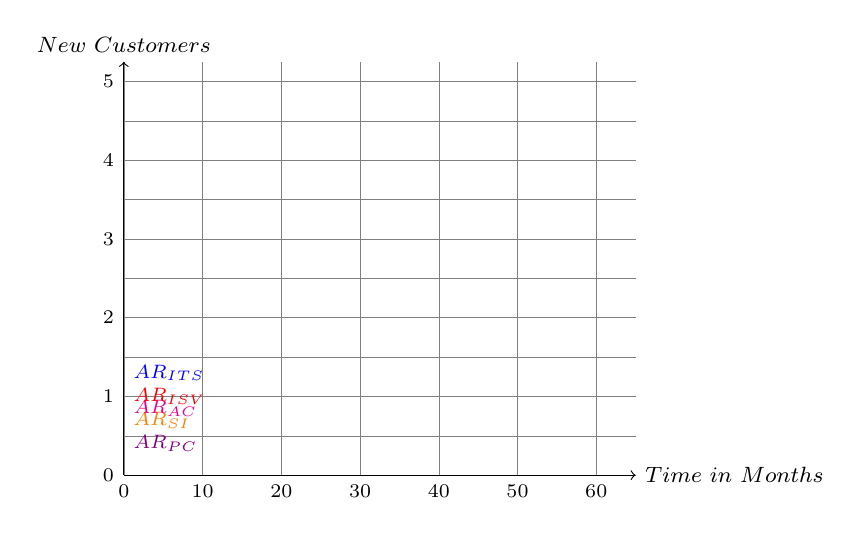
\begin{tikzpicture}[x=0.1cm,y=1cm]

  \def\xmin{0}
  \def\xmax{65}
  \def\ymin{0}
  \def\ymax{5.25}

  % grid
  \draw[style=help lines, ystep=0.5, xstep=10] (\xmin,\ymin) grid
  (\xmax,\ymax);

  % axes
  \draw[->] (\xmin,\ymin) -- (\xmax,\ymin) node[right] {\footnotesize $Time~in~Months$};
  \draw[->] (\xmin,\ymin) -- (\xmin,\ymax) node[above] {\footnotesize $New~Customers$};

  \foreach \x in {0,10,...,60}
    \node at (\x, \ymin) [below] {\scriptsize \x};
  \foreach \y in {0,1,...,5}
    \node at (\xmin,\y) [left] {\scriptsize \y};

  %,mark=*,mark size=0.5pt
	\draw[color=orange] plot[smooth] file {simulationData/SI/adoptionSI.txt}
			node [above=0.7cm, right] {\scriptsize $AR_{SI}$};
	\draw[color=violet] plot[smooth] file {simulationData/PC/adoptionPC.txt}
			node [above=0.4cm, right] {\scriptsize $AR_{PC}$};
	\draw[color=magenta] plot[smooth] file {simulationData/AC/adoptionAC.txt}
			node [above=0.85cm, right] {\scriptsize $AR_{AC}$};
	\draw[color=red] plot[smooth] file {simulationData/ISV/adoptionISV.txt}
			node [above=1.0cm, right] {\scriptsize $AR_{ISV}$};
	\draw[color=blue] plot[smooth] file {simulationData/ITS/adoptionITS.txt}
			node [above=1.3cm, right] {\scriptsize $AR_{ITS}$};										
		
\end{tikzpicture}

	\caption{Proof of Concept Simulation -- New Customers}
\end{figure}


